\section{Molekülorbitale}
\authors{Isabelle Schulte-Herbrüggen, Lena Trahe, Lynn Meeder, Selin Güler}

Die Molekülorbitaltheorie wird genutzt, um die Bindungen innerhalb eines Moleküls quantenmechanisch zu beschreiben. Im Folgenden wird die Theorie auf das Ammoniak- und das Methan-Molekül angewandt.

\subsection{HOMO und LUMO -- freie Elektronenpaare}

Farbigkeit entsteht durch die Absorption von Licht bestimmter Wellenlängen. Diese Wellenlänge wiederum hängt von der Differenz der Energien der verschiedenen Zustände, die man mit den Molekülorbitalen in Näherung beschreiben kann, ab. 
Die Absorption des Lichtes kann man sich als Anregung eines Valenzelektrons in das nächsthöhere Energieniveau vorstellen. Dabei bezeichnet HOMO (Highest Occupied Molecular Orbital) das höchstgelegene besetzte Energieniveau und LUMO (Lowest Unoccupied Molecular Orbital) das nächsthöher gelegene, erste unbesetzte Energieniveau vor der Absorption. Mithilfe des ADF-Programms können sowohl Moleküle gezeichnet als auch Energien berechnet werden. Die Moleküle wurden mit DFT (DZ/B3LYP) berechnet und die Molekülgeometrie wurde mit einem Kraftfeld optimiert.

\begin{dsafigure}
	\centering
	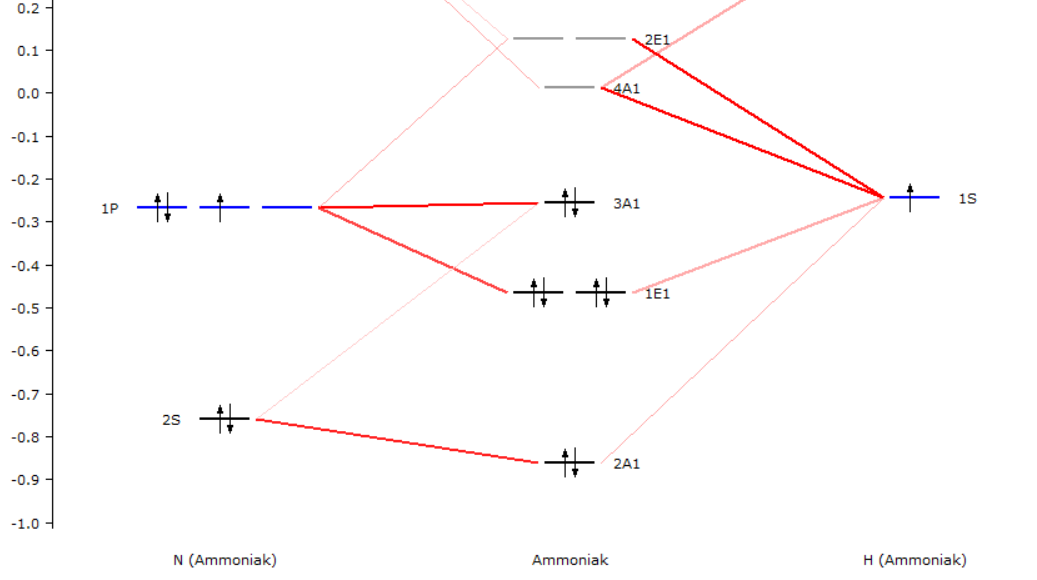
\includegraphics[width=\columnwidth]{AmmoniakLevels.png}
	\caption{Die Energieniveaus der Molekülorbitale von $NH_3$ \cite{ADF2017authors}.}
	\label{levels}
\end{dsafigure}

In Abbildung \ref{levels} sind die verschiedenen Energieniveaus der Molekülorbitale von Ammoniak dargestellt. Links sieht man die Atomorbitale des Stickstoffs, rechts sieht man die Atomorbitale des Wasserstoffs und in der Mitte befinden sich die Molekülorbitale des Ammoniaks. Abbildung \ref{homo} zeigt das höchste besetzte Orbital (HOMO), welches in diesem Fall eine $A_1$-Symmetrie aufweist. Es beschreibt das freie, nicht bindende Elektronenpaar des Ammoniaks. Das erste unbesetzte, energetisch über dem HOMO liegende Orbital ist das beim Ammoniak das ebenfalls $A_1$-Symmetrie aufweisende LUMO, welches in Abbildung \ref{lumo} dargestellt ist.

\begin{dsafigure}
	\centering
	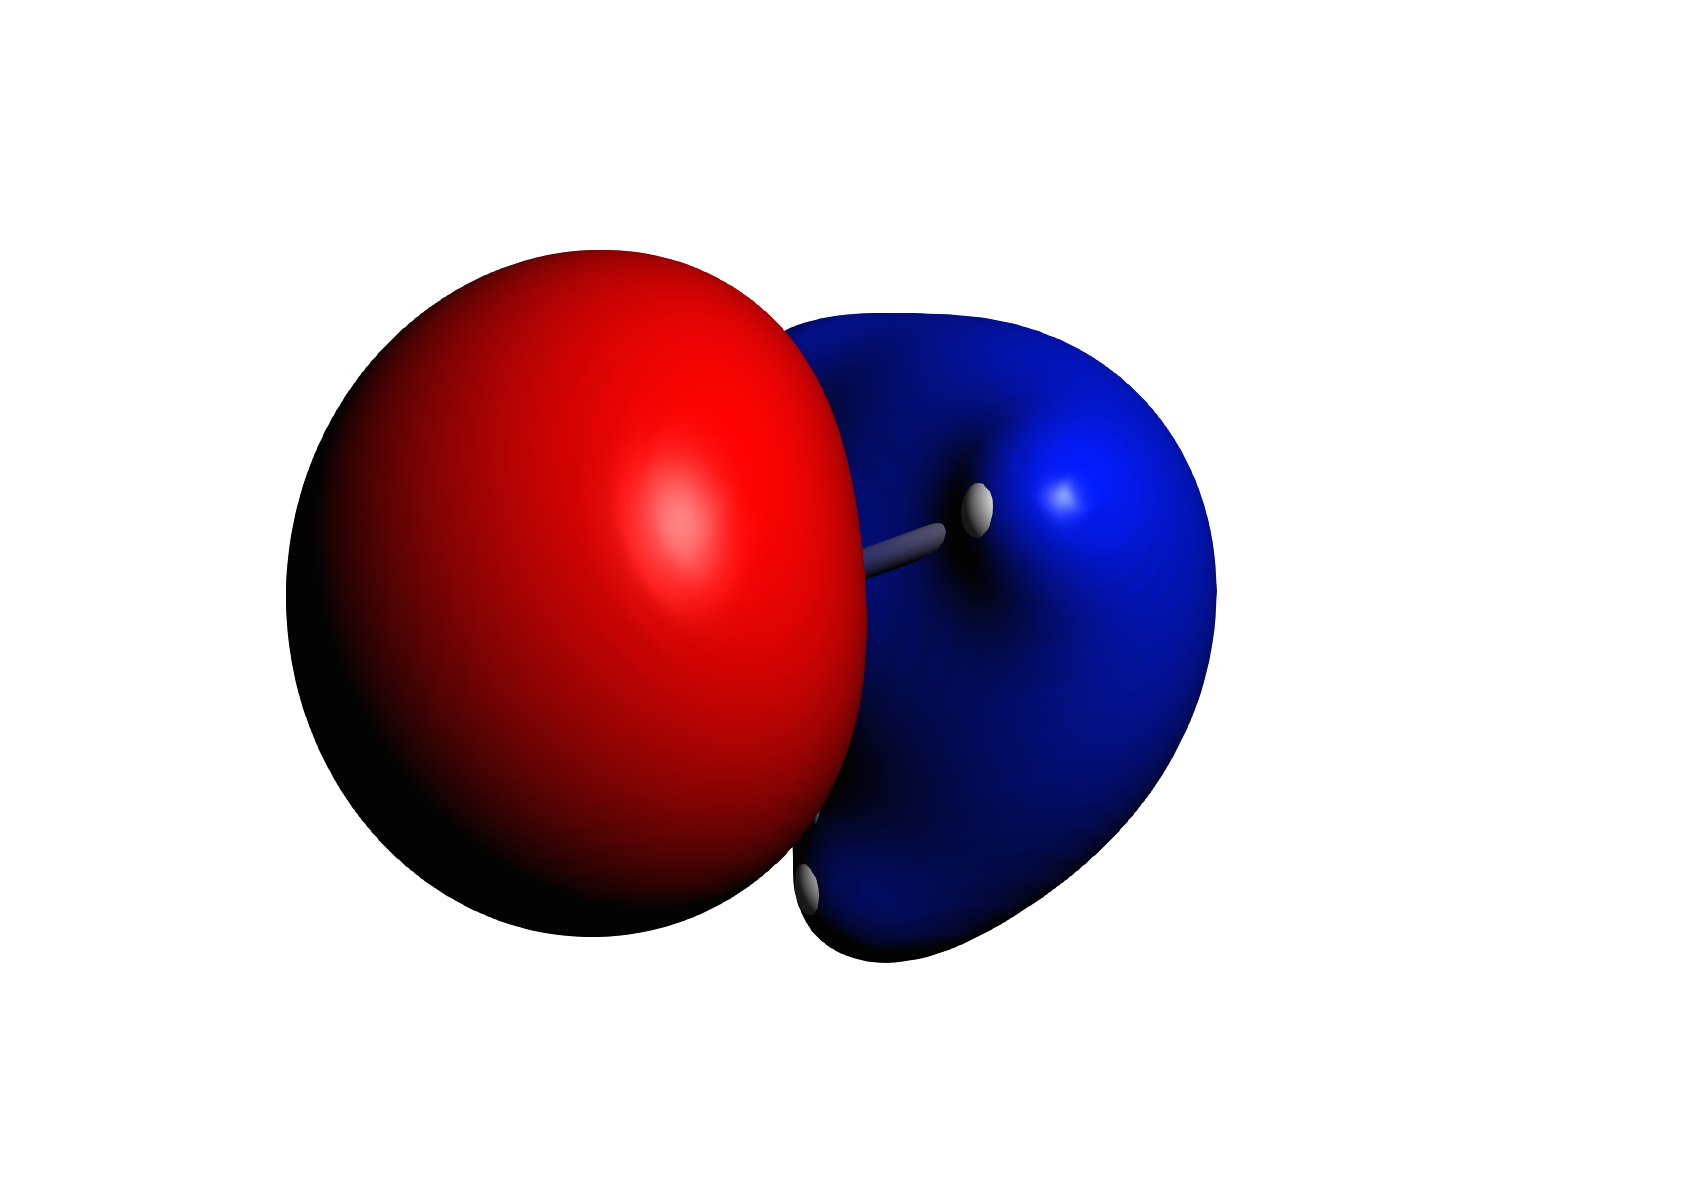
\includegraphics[width=4cm]{Orbital_3A1.png}
	\caption{HOMO des $NH_3$ \cite{ADF2017authors}.}
	\label{homo}
\end{dsafigure}

\begin{dsafigure}
	\centering
	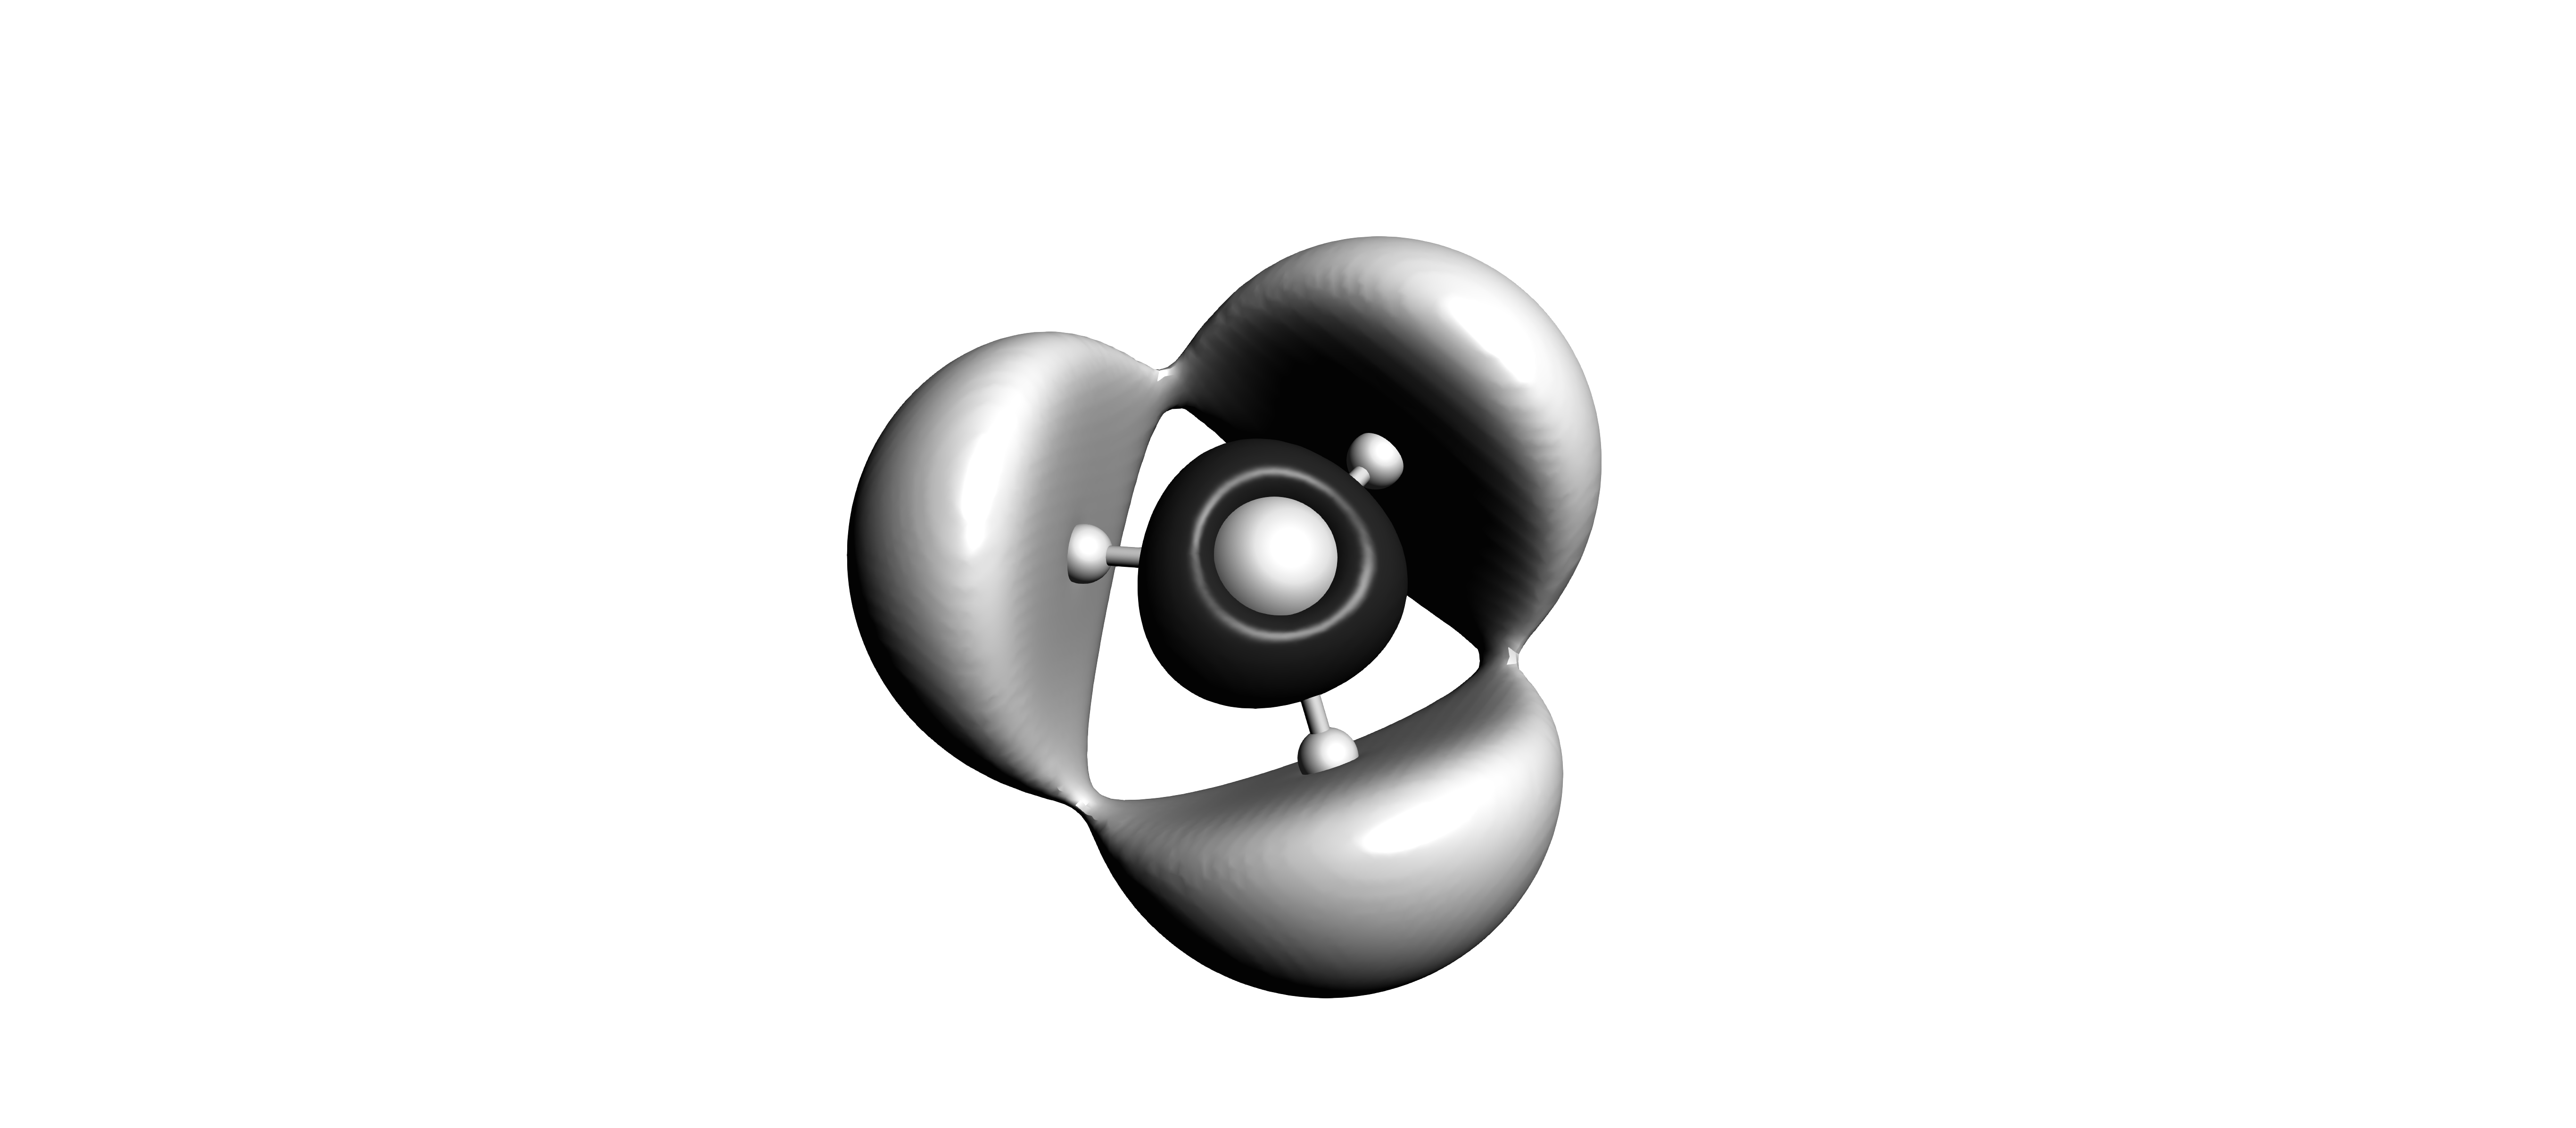
\includegraphics[width=4cm]{Orbital_4A1.png}
	\caption{LUMO des $NH_3$ \cite{ADF2017authors}.}
	\label{lumo}
\end{dsafigure}

\subsection{Hybridisierung versus Molekülorbitaltheorie}

In zahlreichen Experimenten zur Bestimmung von Winkeln und Bindungsabständen wurde belegt, dass ein Methanmolekül die Form eines Tetraeders besitzt. Alle Bindungen sind somit identisch.
Die Berechnung eines Methanmoleküls zeigte einen Unterschied zwischen den Energieniveaus der vier höchsten besetzten Molekülorbitale. Die Abbildung \ref{EnergieniveausMethan} verdeutlicht dies.

\begin{dsafigure}
 \centering
 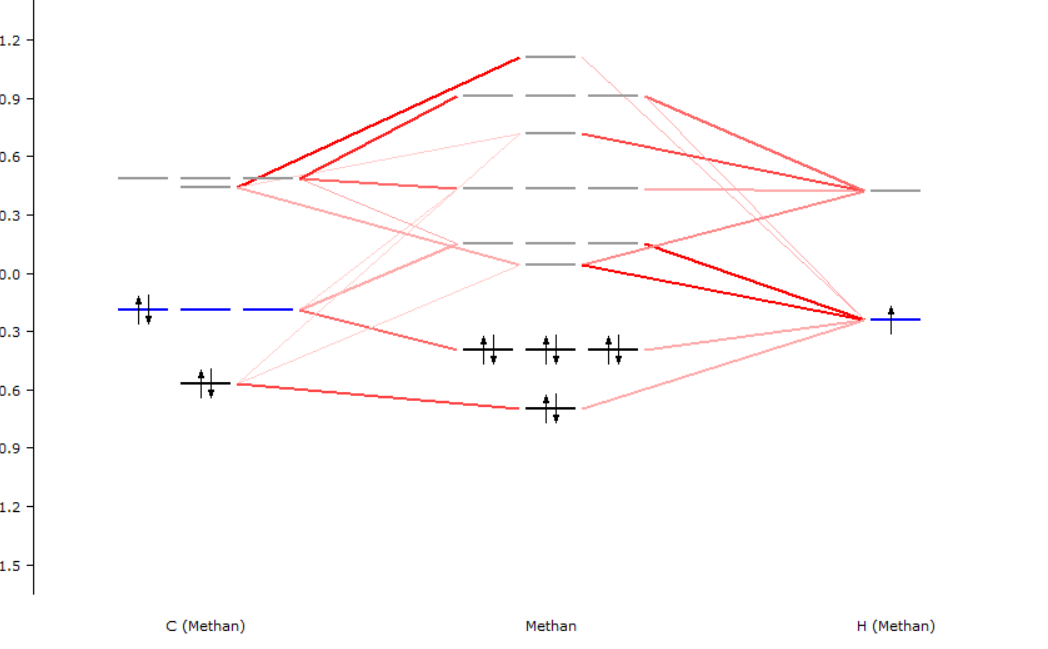
\includegraphics[width=\columnwidth]{LevelsMethan.png}
 \caption{Energieniveaus des Methanmoleküls \cite{ADF2017authors}.}
 \label{EnergieniveausMethan}
\end{dsafigure}

Links sind die Atomorbitale eines Kohlenstoffatoms und rechts die Atomorbitale eines Wasserstoffatoms abgebildet. In der Mitte sind dann die Molekülorbitale des Methanmoleküls dargestellt. Die horizontalen Linien repräsentieren die Energieniveaus der verschiedenen Orbitale. Dabei wird deutlich, dass ein Molekülorbital eine geringere Energie als die übrigen drei der vier höchsten besetzten Molekülorbitale besitzt. 
Es zeigt sich ein Unterschied zwischen dem Modell der Hybridorbitale und der von ADF genutzten Molekülorbitaltheorie, durch die man auch quantitative Informationen wie die Energien erhält. Das Modell der Hybridorbitale hingegen definiert die Energien nicht, sondern liefert qualitative Aussagen zur Geometrie und Bindungsverhältnissen. Hybridorbitale resultieren bloß aus der Anpassung der Atomorbitalbasis an die Tertaederstruktur des Moleküls. Für die Molekülorbitale werden hingegen die Energien einzelner Elektronen optimiert. 
Es handelt sich also um zwei unterschiedliche Betrachtungsweisen.
Insgesamt beschreiben beide Modelle die Struktur des Methanmoleküls als Tetraeder. In Abbildung \ref{OrbitalMethan} ist eins der drei HOMOs dargestellt.

\begin{dsafigure}
 \centering
 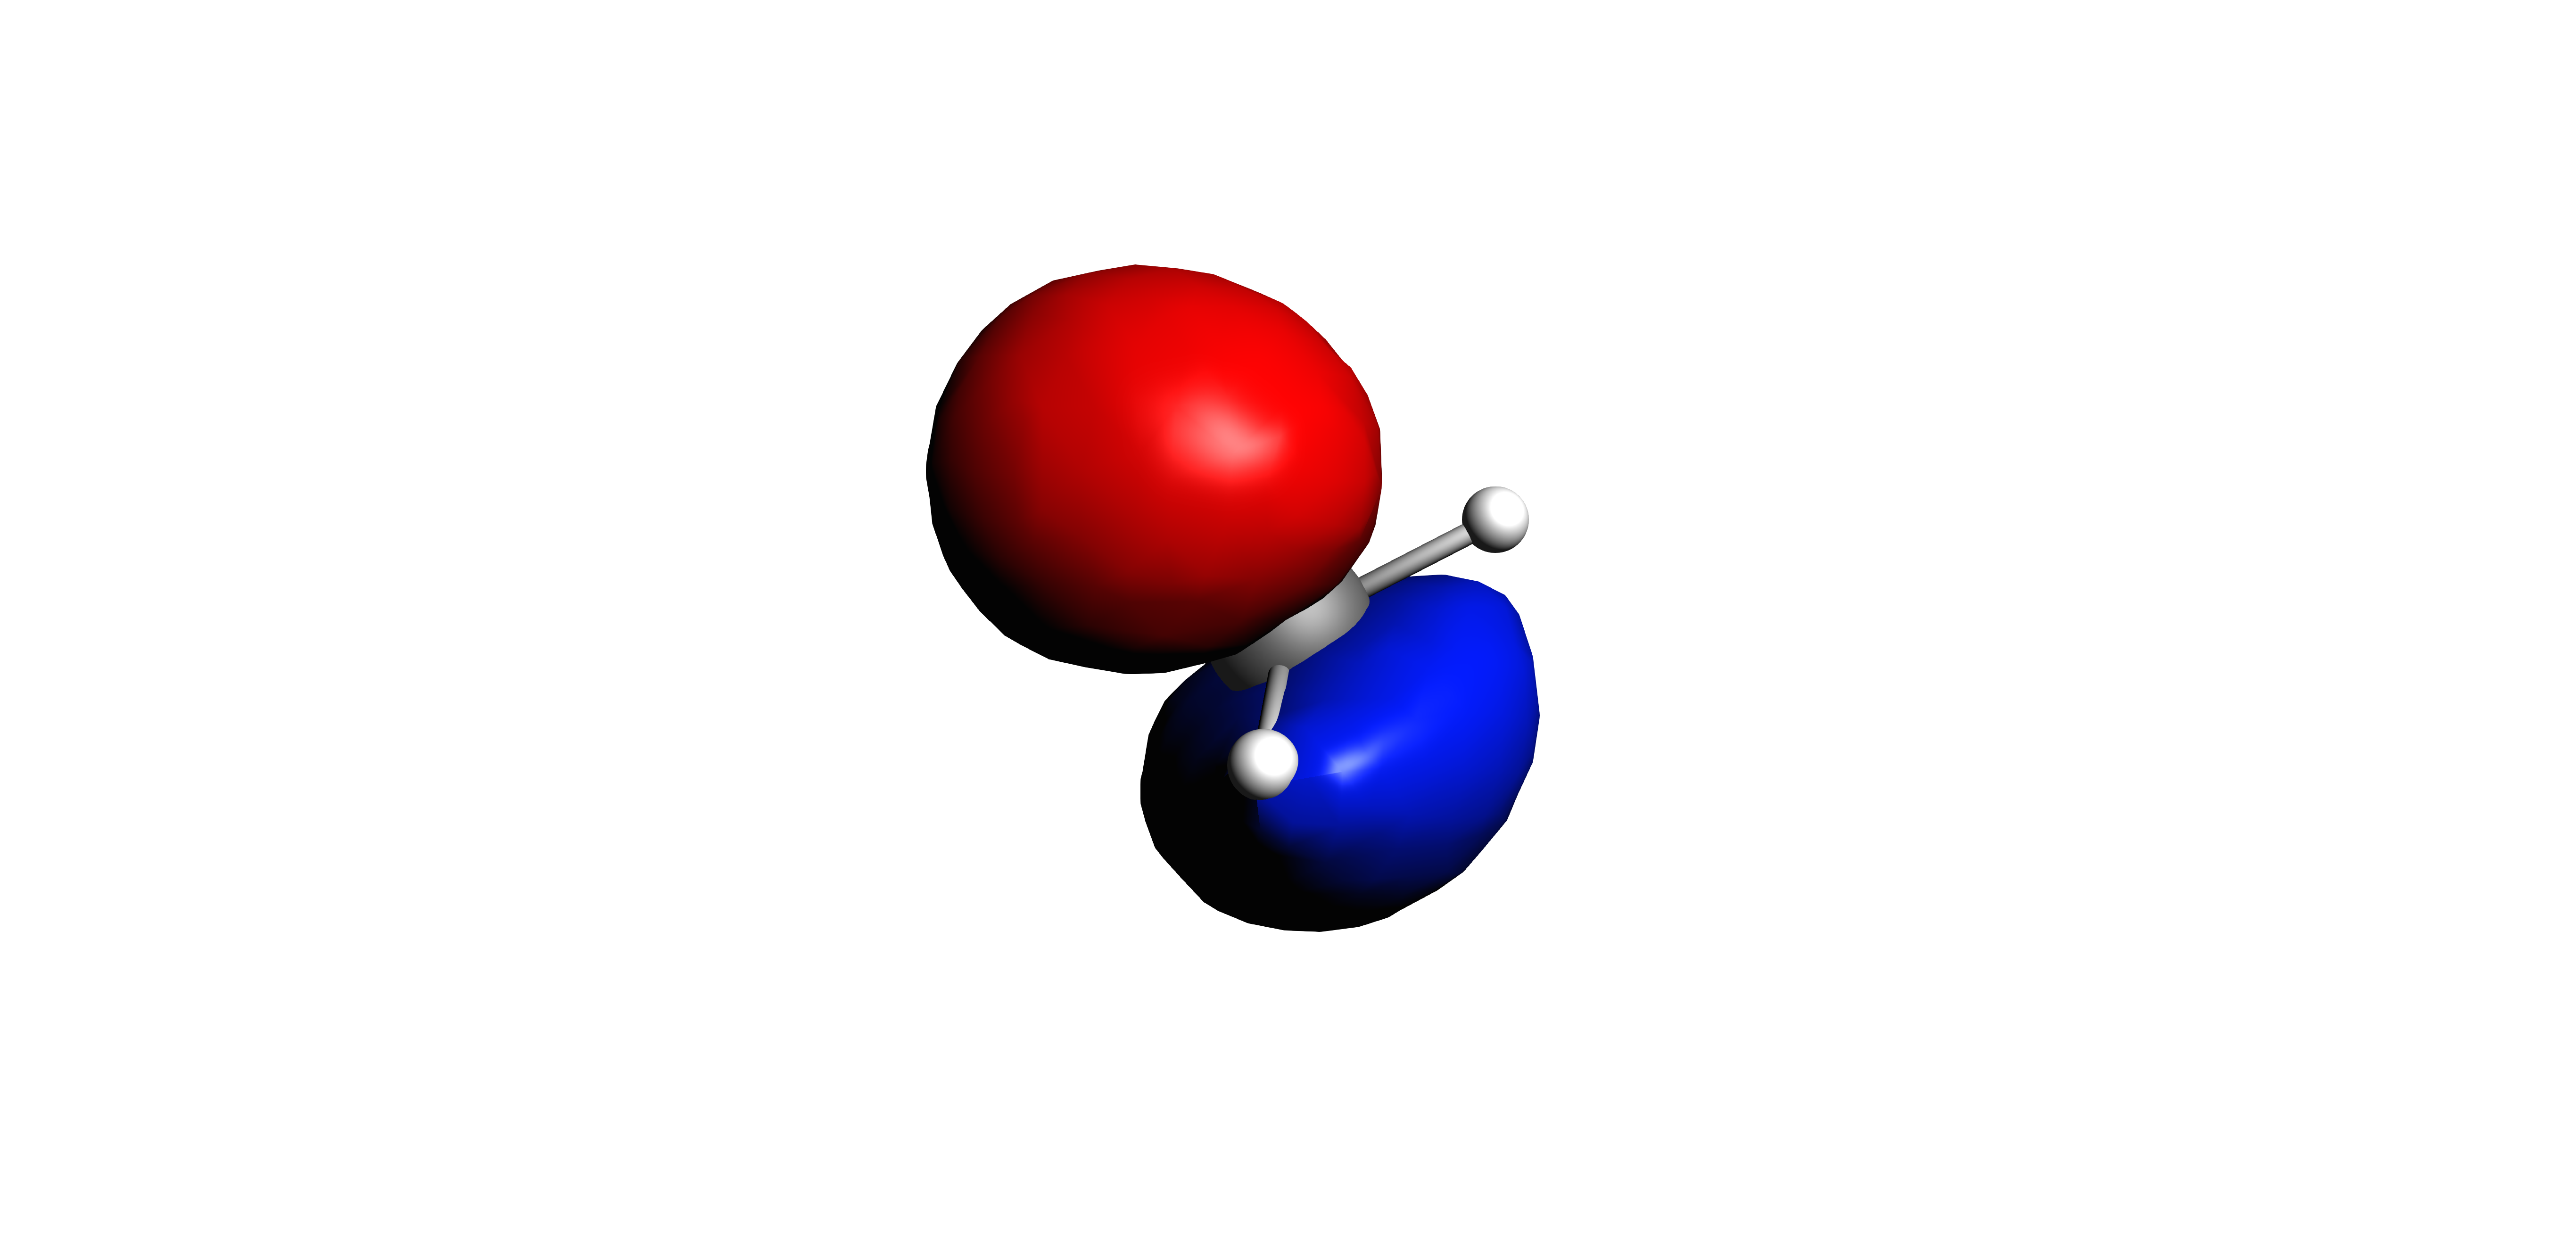
\includegraphics[scale=0.04]{MethanA5.png}
 \caption{Eines der drei HOMOs eines Methanmoleküls \cite{ADF2017authors}.}
 \label{OrbitalMethan}
\end{dsafigure}

